\documentclass[12pt]{article}
\usepackage[a4paper,margin=1in]{geometry}
\usepackage{graphicx}
\usepackage{caption}
\usepackage{subcaption}
\usepackage{amsmath}
\usepackage{float}
\usepackage{authblk}
\usepackage{siunitx}
\usepackage{hyperref}
\hypersetup{
	colorlinks   = false,    
	pdfborder    = {0 0 0}, 
	hidelinks    = true      
}

\usepackage{booktabs}


\title{\textbf{Cosmic Ray Detection Using Smartphone CMOS Sensor Data}} 
\author[]{Mufeez}
\author[]{Zahra}
\author[]{Muzammil Shah}
\affil[]{Department of Physics, Quaid-i-Azam University}
\date{\today}


\begin{document}
	\maketitle	
	
	\begin{abstract}
		This report details an experiment to detect cosmic-ray muons using images captured by a smartphone CMOS sensor and pre-processed by the SoraMame app. Data collected over \SI{42847.6}{\second} yielded \num{128} events. We analyze temporal and spatial distributions, estimate the muon flux, and validate the random arrival assumption using Poisson statistics.
	\end{abstract}
	

	\section{Detection Mechanism}
	When a charged particle, such as a cosmic ray muon, traverses the depleted region of a CMOS (complementary metal–oxide–semiconductor) image sensor, it deposits energy along its path. This energy ionises the silicon substrate, generating electron–hole pairs, which are subsequently collected and registered as discrete signals. However, smartphone CMOS sensors are not optimised for high-energy particle detection: their small pixel area and low signal-to-noise ratio, particularly at high ISO values, introduce significant challenges. Thermal noise, hot pixels, and electronic readout fluctuations can easily mimic particle-like events. To address this, the SoraMame application implements a dynamic intensity thresholding algorithm to distinguish genuine ionisation tracks from background noise. While effective at suppressing spurious signals, this method is not foolproof: it may exclude low-energy events or misclassify high-noise artefacts, thus imposing a trade-off between detection efficiency and purity.
	
	\section{Data Acquisition via SoraMame App}
	
	The SoraMame app transforms a smartphone's CMOS camera sensor into a basic cosmic-ray detector. In dark-field conditions (e.g., lens covered or placed in a lightproof box), the app continuously captures images, monitoring pixel intensities for transient, high-energy spikes characteristic of charged particle tracks.
	
	When such a spike exceeds a predefined threshold, the app flags the frame as a candidate event. These candidate images, along with relevant metadata (timestamp, sensor model, exposure time), are uploaded to the SoraMame central database. Users can retrieve their data in .csv format via their web dashboard.
	
	For this project, the event dataset was exported from the official SoraMame portal as a .csv file containing pixel coordinates, timestamps, and device identifiers.
	
\begin{figure}[H]
	\centering
	\begin{subfigure}[b]{0.45\textwidth}
		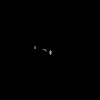
\includegraphics[width=\textwidth]{../Data and notebooks/figures/Sample images/2025-07-2406_07_38.102220_3451-2051.png}
		\caption{}
		
	\end{subfigure}
	\hfill
	\begin{subfigure}[b]{0.45\textwidth}
		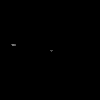
\includegraphics[width=\textwidth]{../Data and notebooks/figures/Sample images/2025-07-2406_23_25.381925_1572-2397.png}
		\caption{}
	\end{subfigure}
	\vspace{0.5em}
	
	\begin{subfigure}[b]{0.45\textwidth}
		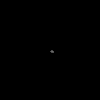
\includegraphics[width=\textwidth]{../Data and notebooks/figures/Sample images/2025-07-2407_03_18.346530_405-1571.png}
		\caption{}
	\end{subfigure}
	\hfill
	\begin{subfigure}[b]{0.45\textwidth}
		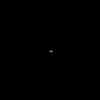
\includegraphics[width=\textwidth]{../Data and notebooks/figures/Sample images/2025-07-2407_05_26.138612_3924-1241.png}
		\caption{}
	\end{subfigure}
	
	\caption{Sample cosmic-ray event frames captured using the SoraMame app. High-energy charged particles appear as bright streaks or spots on the sensor.}
	\label{fig:soramame_grid}
\end{figure}

	
	\section{Flux Estimation}
	The flux $\Phi$ is defined as:
	\begin{equation}
		\Phi = \frac{N}{A\,t}
	\end{equation}
	where:
	\begin{itemize}
		\item $N = 128$ is the total event count,
		\item $A = \SI{0.2048}{cm^2}$ is the active sensor area,
		\item $t = \SI{42847.6}{s}$ is the net observation time.
	\end{itemize}
	Substituting,
	\[
	\Phi = \frac{128}{0.2048 \times 42847.6} = \SI{1.4587e-2}{events/cm^2/s} = \SI{0.8752}{events/cm^2/min}.
	\]
	
	Typical ground-level muon flux is $\sim\SI{1}{event/cm^2/min}$; our measured value falls within statistical and environmental uncertainties.
	
	\section{Poisson Distribution}
	Muon arrivals are independent and occur at a constant average rate, justifying modeling by a Poisson process. The probability of $k$ events in interval $T$ is:
	\[
	P(k;\lambda) = \frac{\lambda^k e^{-\lambda}}{k!}
	\]
	where $\lambda = \bar{N}_T$ is the mean count per interval.
	
	\section{Data Preprocessing}
	For the data analysis we used python with these packages:
	 \begin{itemize}
	 	\item Pandas (For dealing with .csv data)
	 	\item Matplotlib (For plotting our data)
	 	\item numpy (For mathematical calculations)
	\end{itemize}
	
	\section{Temporal Binning}
	\begin{itemize}
		\item Hourly counts: resampled to one-hour bins. Additionally, half-hour bins were used for improved resolution in the Poisson distribution analysis (see Figure~\ref{fig:poissonhalfhour}).
		\item Cumulative counts: minute-by-minute cumulative sum.
	\end{itemize}
	
	\section{Statistical Analysis}
	\begin{enumerate}
		\item Mean hourly count $\lambda = 10.67$ events/h.
		\item Mean Half hour count $\lambda= 5.33$ events/30min.
		\item Poisson PMF calculated for $k=0\ldots16$ using \texttt{scipy.stats.poisson}.
	\end{enumerate}
	
	\section{Results and Discussion}
	
	\subsection{Hourly Event Counts}
	\begin{figure}[H]
		\centering
		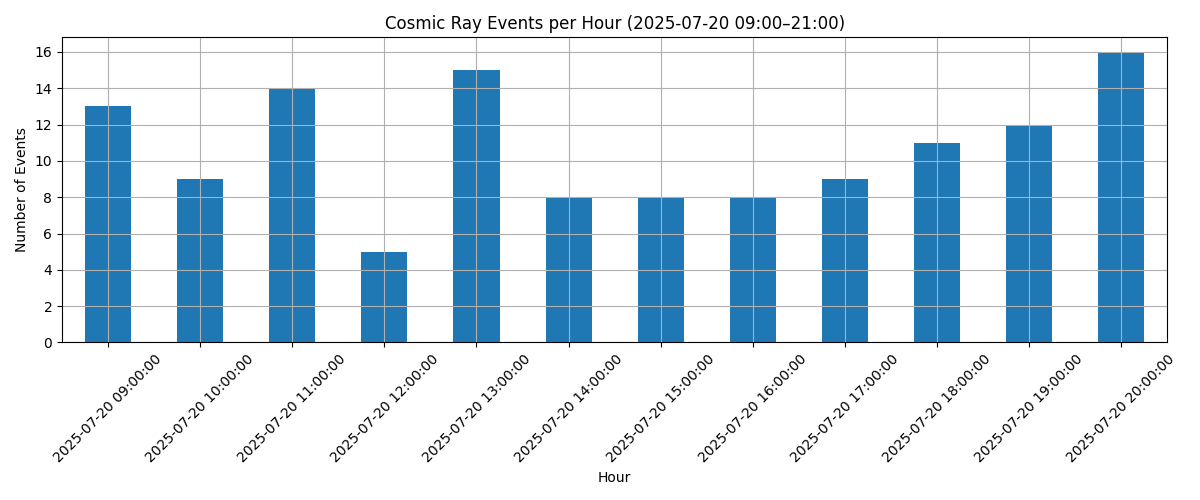
\includegraphics[width=0.9\textwidth]{../Data and notebooks/figures/events_per_hour.png}
		\caption{Hourly cosmic-ray event counts from 09:00 to 20:00.}
		\label{fig:hourly}
	\end{figure}
	
	The plot in Figure~\ref{fig:hourly} shows counts ranging from 5 to 16 per hour. The most active hour (20:00–21:00) recorded 16 events, slightly above the mean, while midday counts dipped to 5 events at 12:00.
	
	\subsection{Cumulative Event Trend}
	\begin{figure}[H]
		\centering
		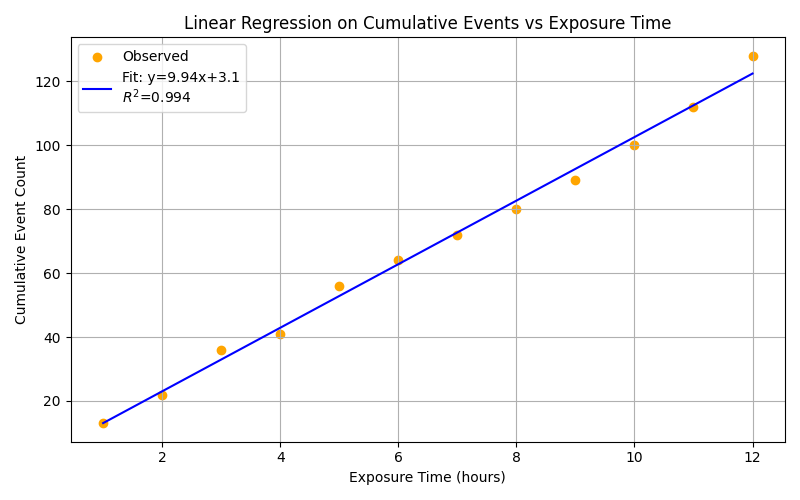
\includegraphics[width=0.9\textwidth]{../Data and notebooks/figures/linear regression Cum-events vs Exp time.png}
		\caption{Cumulative count of events versus time.}
		\label{fig:cumulative}
	\end{figure}
	
	Figure~\ref{fig:cumulative} demonstrates an overall linear increase in total events.
	
	\subsection{Poisson Distribution Fit}
	\begin{figure}[H]
		\centering
		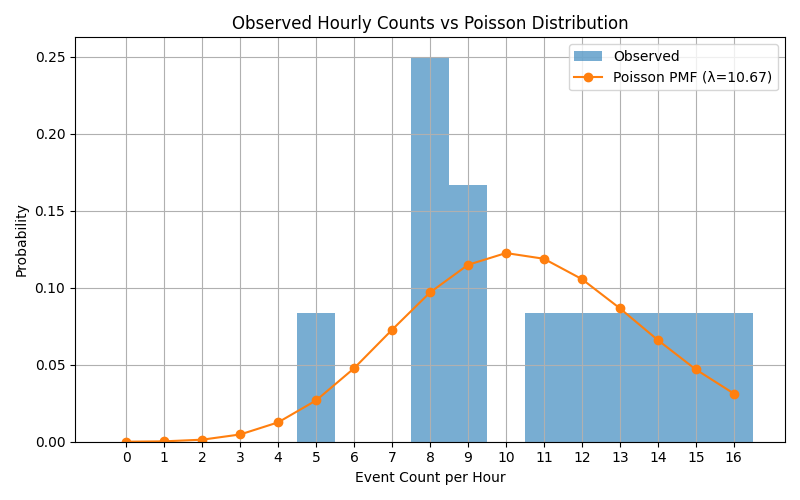
\includegraphics[width=0.9\textwidth]{../Data and notebooks/figures/poisson_fit_hourly_counts.png}
		\caption{Histogram of observed hourly counts (normalized) overlaid with Poisson PMF for $\lambda=10.67$.}
		\label{fig:poisson}
	\end{figure}
	
	\begin{figure}[H]
		\centering
		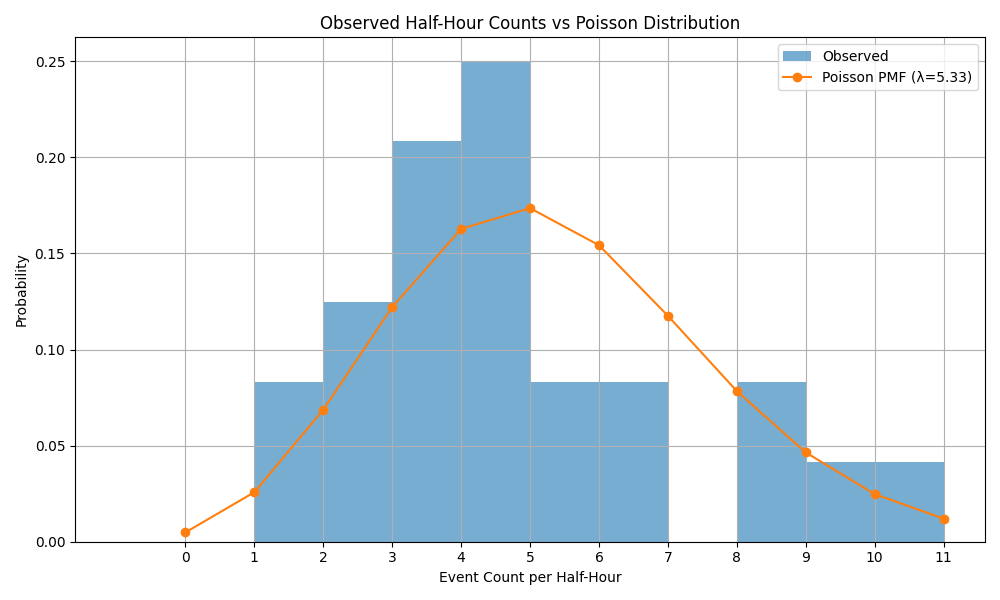
\includegraphics[width=0.9\textwidth]{../Data and notebooks/figures/poisson_fit_halfhourly_counts.png}
		\caption{Histogram of observed half hour counts (normalized) overlaid with Poisson PMF for $\lambda=5.33$.}
		\label{fig:poissonhalfhour}
	\end{figure}
	
	Figure~\ref{fig:poisson} shows the normalized histogram of counts alongside the theoretical Poisson probabilities. However, the distribution does not align perfectly with the observed data. This discrepancy arises because hourly binning is a coarser grouping, which can obscure finer variations in the event counts.
	
	
	Figure~\ref{fig:poissonhalfhour} shows half-hour bins, which provide better resolution. With the recalculated $\lambda = 5.33$, the observed event distribution exhibits closer agreement with the expected Poisson model.
	
	
	
	\subsection{Spatial Distribution}
	\begin{figure}[H]
		\centering
		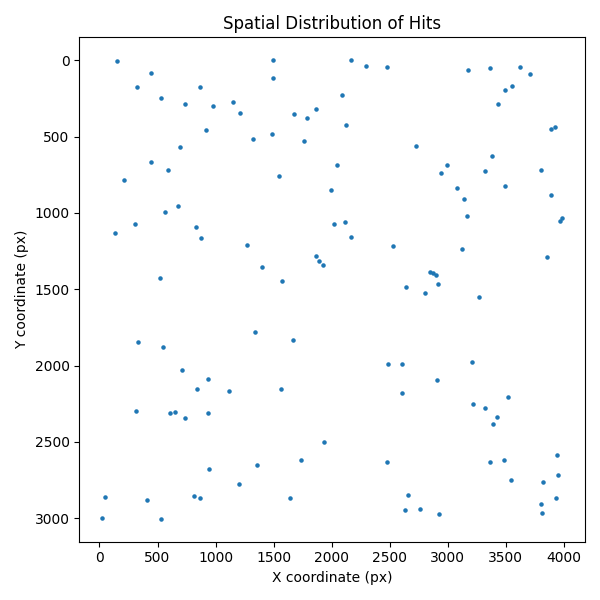
\includegraphics[width=0.75\textwidth]{../Data and notebooks/figures/spatial_distribution.png}
		\caption{Scatter of hit coordinates on the CMOS sensor. Uniform coverage indicates no sensor bias or localized noise artifacts.}
		\label{fig:spatial}
	\end{figure}
	
	Spatial uniformity in Figure~\ref{fig:spatial} implies consistent sensitivity across the sensor, validating the threshold choice and dark-field imaging setup.
	
	\section{Conclusion}
	This experiment successfully detected cosmic-ray muons using smartphone CMOS dark frames and analyzed their statistics. The measured flux \SI{0.8752}{events/cm^2/min} closely matches expected values. Half hour variations conform to Poisson distribution, and spatial mapping reveals no detector bias. Future work could extend observation duration. A better self learning model would easily filter the candidate events more accurately than our current filtering models.
	
	\pagebreak
	\noindent\textbf{Code and Data Repository:} The full data analysis pipeline, including CSV parsing, plotting scripts, and this report's LaTeX source, is available at:
	
	\url{https://github.com/Mufeez-dev/cosmic-ray-detection-using-soramame-data}
	
	\section*{References}
	\begin{enumerate}
		\item Vandenbroucke, J. et al. (2016). *Measurement of cosmic-ray muons with the Distributed Electronic Cosmic-ray Observatory, a network of smartphones.* [JINST 11 (2016) P04019].\\
		\url{https://ui.adsabs.harvard.edu/abs/2016JInst..11P4019V/abstract}
		
		\item Swaney, J. et al. (2021). *Measurement of Smartphone Sensor Efficiency to Cosmic Ray Muons.*\\
		\url{https://arxiv.org/abs/2107.06332}
		
		\item Pérez, M. et al. (2016). *Particle detection and classification using commercial off-the-shelf CMOS image sensors.* [Nucl. Instrum. Meth. A 827 (2016) 171–180].\\
		\url{https://ui.adsabs.harvard.edu/abs/2016NIMPA.827..171P/abstract}
		
		\item Winter, M. et al. (2018). *Particle Identification in Camera Image Sensors Using Computer Vision.*\\
		\url{https://www.researchgate.net/publication/323746988_Particle_Identification_In_Camera_Image_Sensors_Using_Computer_Vision}
	\end{enumerate}
	
	
	
	
\end{document}
